\lab{Introduction to Matplotlib: 3D Plotting and Animations}{Introduction to Matplotlib: 3D Plotting and Animations}
\label{lab:lab0}

\objective{Animations and 3D plots are useful in visualizing solutions to ODEs and PDEs found in many dynamics and control problems.
In this lab we explore the functionality contained in the 3D plotting and animation libraries in Matplotlib.}
 
\section*{Introduction}
Matplotlib is a Python library that contains tools for creating plots in multiple dimensions.
The library contains important classes that are needed to create plots.
The most important objects to understand in this lab are figure objects, axes objects, and line objects. These three objects are created using the following code.

\begin{lstlisting}
>>> import matplotlib.pyplot as plt
>>> fig = plt.figure()                  # Create figure object.
>>> ax = fig.add_subplot(111)           # Create axes object.
>>> line2d, = plt.plot([],[])           # Create empty 2D Line object
>>> line3d, = plt.plot([],[],[])        # Create empty 3D line object
\end{lstlisting}

Recall that \li{plt.figure()} creates a \li{matplotlib.figure.Figure} object, which is the window that is displayed when \li{plt.show()} is called.
3D plotting and animation both require explicitly defining the \li{Figure} object, as shown above.
This allows for the object to be updated and modified, as will be explained later in the lab.

\li{Figure} objects contain \li{matplotlib.axes._subplots.AxesSubplot} objects, called \textit{axes}. Axes are spaces to plot on, and are created by the \li{add_subplot()} method of a \li{Figure} object. Figures can have multiple axes. 
%For more information, see [reference Intro to Matplotlib 1 here].

Calling \li{plt.plot()} returns a list of line objects.
For example, supposing \li{x1}, \li{y1}, \li{x2}, and \li{y2} are arrays containing data for two separate curves, then calling \li{plt.plot(x1, y1, x2, y2)} will return a list with two elements.
Each element of the list is a \li{matplotlib.lines.Line2D} object.
If the axes is three-dimensional, then the returned list will contain \li{matplotlib.lines.Line3D} objects.
Because this function call returns a list, if only one line is plotted, adding a trailing comma to the variable name will assign the name to the first element of the returned list.
You can alternatively reference the zero index of the returned list, but using a trailing comma is standard.

\begin{comment} 
As mentioned in the Introduction to Matplotlib lab in Volume 1, 3D plots and animations are useful in visualizing solutions to ODEs and PDEs found in many dynamics and control problems.
This lab covers basics for 3D plotting, animating 2D plots, and animating 3D trajectories and 3D surfaces. 

In Matplotlib, plots are created using figure objects.
It is possible to create a plot without explicitily instantiating the figure object, but creating an instance separately allows for useful functions to be called on that object. Initializing a figure object is done using the following code:

\begin{lstlisting}
>>> fig = plt.figure()
\end{lstlisting}

3D plotting and animation both require the figure object to be created explicitly. 
\end{comment}
\begin{comment}
\begin{info}
There are different options for plotting in Jupyter Notebook.
In the past we have used \li{\%matplotlib inline}.
For labs with animation we will use \li{\%matplotlib notebook} instead.
This is an interactive regime that allows animations to be displayed without creating a new window.
\end{info}
\end{comment}

\section*{Animation Basics}
The animation library in Matplotlib contains a class called \li{FuncAnimation}.
We will use this class throughout this lab. \li{FuncAnimation} requires a user-defined \textit{update} function that controls the plot for each frame of the animation. 
This grants the user wide flexibility and control of the resulting animation.
The following steps describe the process of creating a simple animated plot using the \li{FuncAnimation} class. 
\begin{enumerate}
\item Compute all data to be plotted.
\item Explicitly define figure object.
\item Define line objects to be altered dynamically.
\item Create function to update line objects.
\item Create \li{FuncAnimation} object.
\item Display using \li{plt.show()}.
\end{enumerate}

These steps will be explained by way of an example.
The arrays \li{x} and \li{y} contain data giving the location of a particle moving in the plane.
To visualize this motion, one could animate the particle as well as display the trajectory that the particle has traveled.
For this animation, two separate \li{Line2D} objects must be created on an axes object.
The first, \li{particle} will be for the position of the particle itself, and the second, \li{traj} will be for the trajectory that the particle has traveled.
Note that these objects are created with empty lists of data.
The update function will be used to dynamically set the data to be plotted in these line objects.

\begin{lstlisting}
>>> import matplotlib.animation as animation
>>> import numpy as np
>>> t = np.linspace(0,2*np.pi,100)
>>> x = np.sin(t)
>>> y = t**2
>>> fig = plt.figure()
>>> ax = fig.add_subplot(111)
>>> ax.set_xlim((-1.1,1.1))
>>> ax.set_ylim((0,40))
>>> particle, = plt.plot([],[], marker='o', color='r')
>>> traj, = plt.plot([],[], color='r', alpha=0.5)
\end{lstlisting}

The update function must be defined a specific way in order to interact properly with the 
\li{matplotlib.animation.FuncAnimation} object.
The update function must accept the current frame index as its first input parameter and it must return a list or tuple of line objects.
The current frame index is used to access the data to be plotted in the current frame. 
Both 2D and 3D line objects have the built-in method \li{.set_data()}.
This function takes in two one-dimensional arrays representing x and y values to plot.
This allows a single line object to display different data for each frame.
Inside the update function, \li{.set_data()} is called on the line objects with the relevant data as inputs.


\begin{lstlisting}
>>> def update(i):
>>>     particle.set_data(x[i],y[i])
>>>     traj.set_data(x[:i+1],y[:i+1])
>>>     return particle,traj
\end{lstlisting}

\begin{comment}
Three main objects are required for animating plots in Matplotlib.
First, you need to create a figure object as explained above.
Then you need to create a \li{matplotlib.lines.Line2D} or \li{matplotlib.lines.Line3D} object (depending on the dimension of the graph you are animating).
The following code shows one way to initialize a \li{Line2D} object:

\begin{lstlisting}
>>> line, = plt.plot([],[])
\end{lstlisting}

As explained above, \li{plt.plot()} returns a list.
Thus setting the output equal to \li{line,} is equivalent to setting the variable named \li{line} to the first element of the returned list.
Accessing the zero index of the list would yield the equivalent result, but it is conventional to use the trailing comma.

One figure and line objects have been initialized, an update function needs to be defined and a \li{FuncAnimation} object created.
The \li{FuncAnimation} constructor takes in the figure and the update function as inputs.
It calls the update function at each frame of the animation. 

The update function must take the time frame index as its first parameter.
The \li{Line2D} and \li{Line3D} objects have the built in function call \li{set_data()}.
This function takes in 2 1D arrays representing x and y values (or a 2xn array with x and y values). Inside the update function, the \li{set_data()} function is called on the line objects using the frame index to specify the data.
Then the line object is returned, as shown below:

\begin{lstlisting}
>>> def update(i):
>>>     line.set_data(x, y[i])
>>>     return line,
\end{lstlisting}
\end{comment}

Next, the \li{FuncAnimation} object is created.
The argument \li{frames} specifies the iterable representing the frame indices.
If \li{frames} is an integer, it is treated as the iterable \li{range(frames)}.
After the \li{FuncAnimation} object is created, \li{plt.show()} displays the animation.

\begin{lstlisting}
>>> ani = FuncAnimation(fig, update, frames=range(100), interval=25)
>>> plt.show()
\end{lstlisting}

The following table shows more parameters that can be passed into FuncAnimation.

\begin{table}[H]
\centering
\begin{tabular}{r|l}
Parameter & Description\\
\hline
\li{fargs} (tuple) & Additional arguements to pass update function\\
\li{interval} (float) & Delay between frames in milliseconds\\
\li{repeat} (bool) & Determines whether animation repeats (Default True)\\
\li{blit} (bool) & Determines whether blitting is used (Default False)\\
\end{tabular}
\end{table}

\begin{info}
When using FuncAnimation, it is essential that a reference is kept to the instance of the class.
The animation is advanced by a timer and if a reference is not held for the object, \li{Python} will automatically garbage collect and the animation will stop.
\end{info}

\subsubsection*{Saving Animations}
The simplest way to save an animation is to encode it to a \li{.mp4} file, which will allow you to display the video inline inside a Jupyter Notebook, or view it using any video player supporting the chosen filetype.

Unfortunately, Matplotlib does not come with a built-in video encoder.
The \li{matplotlib.animation} module supports several third-party encoders. FFmpeg is a lightweight solution which can be obtained from \href{https://www.ffmpeg.org/download.html}{https://www.ffmpeg.org/download.html}.
When available, FFmpeg is generally chosen as the default, but you may need to specify to Matplotlib to use it:
\begin{lstlisting}
animation.writer = animation.writers['ffmpeg']
\end{lstlisting}

To prevent the animation from displaying while it is being rendered as video, use \li{plt.ioff()}.
This turns off matplotlib's interactive mode until \li{plt.ion()} is called.
After creating the animation object, use its \li{.save()} method with the desired filename to render and save the video. The following code is given for reference:

\begin{lstlisting}
plt.ioff()    # Turn off interactive mode to hide rendering animations

# Code to create figure, axes, and update function goes here
# ...
ani = animation.FuncAnimation(fig, update, frames, interval)
ani.save('my_animation.mp4')
\end{lstlisting}
To display the \li{.mp4} video in a Jupyter Notebook, place the following HTML code in a separate markdown cell:
\begin{lstlisting}
<video src="my_animation.mp4" controls>
\end{lstlisting}

\subsection*{Embedding Animations}
While saving animations to a file has the advantage that the animation will persist if the notebook is closed and reopened, it tends to be much slower than directly embedding the animation in the notebook.
Directly embedding can thus be useful in the process of creating an animation by allowing faster experimentation.

After creating an animation, calling \li{plt.show()} will attempt to embed it; however, some systems may struggle to display an animation in this way.
When this is the case, it may be easier to embed the animation using the HTML5 API. 
Jupyter notebooks use HTML to display their contents, so we can leverage this and use HTML5's video capabilities to insert video directly into a notebook.

To embed the video directly into a notebook using HTML5 you must use the \li{IPython.display} module.
This module will be able to interpret an encoded HTML5 video, which \li{matplotlib.animation} can create.
This method tends to be much more simple than rendering the animation to an \li{.mp4} file and then embedding that file into a notebook, as it does not require an outside encoder, and it tends to be encounter fewer bugs than using \li{plt.show()}.
However, the animation generally does not persist if the notebook is closed and reopened.
Here is a snippet you may reference to embed an animation using \li{IPyton.display}
\begin{lstlisting}
# required import statements
from IPython.display import HTML
import matplotlib.pyplot as plt
from matplotlib import animation

# disable interactive mode
plt.ioff()
''' 
Here we would insert whatever code needed to create the animation
such as instantiating the fig object and defining the update function
'''
# create animation
ani = animation.FuncAnimation(fig, update, frames, interval)
# render as html5 and embed
HTML(ani.to_html5_video())
\end{lstlisting}

\begin{warn}
Note that animations that are embedded in the notebook using \li{plt.show()} or \li{HTML()} \textbf{\emph{do not}} persist if the notebook is closed and reopened.
While this method can be useful for more quickly testing animations, \textbf{\emph{do not}} use this method for embedding the final animations of your finished lab, as the grader will not be able to view your animations.
Rather, save the animation to an \li{.mp4} file and embed the created file.
When pushing your lab, be sure to also add and push the video files you create.
\end{warn}

\begin{problem}
Use the FuncAnimation class to animate the function $y=\sin(x+0.1t)$ where $x \in [0,2\pi]$, and $t$ ranges from $0$ to $100$ seconds. 
Save your animation to a file and embed that into the notebook.
\end{problem}

\section*{3D Plotting Introduction}
3D plotting is very similar to 2D plotting.
The main difference is that a set of 3D axes must be created within the figure object.
A 3D axes object is created using the additional keyword argument \li{projection='3d'}:

\begin{lstlisting}
>>> # Create figure object.
>>> fig = plt.figure()
>>>
>>> # Create 3D axis object using add_subplot().
>>> ax = fig.add_subplot(111, projection='3d')
\end{lstlisting}

\subsection*{3D Static Plotting}

When the axes object is explicitly defined, plots are generated by calling the chosen plot function (such as \li{ax.plot()} on the axes object.
Additional information on the use of axes objects can be found here: \href{https://matplotlib.org/api/axes\_api.html}{https://matplotlib.org/api/axes\_api.html}.

\begin{problem}
The orbits for Mercury, Venus, Earth, and Mars are stored in the file \li{orbits.npz}.
The file contains four NumPy arrays: \li{mercury}, \li{venus}, \li{earth}, and \li{mars}.
The first column of each array contains the x-coordinates, the second column contains the y-coordinates, and the third column contians the z-coordinates of each planet, all relative to the Sun, and expressed in AU (astronomical units, the average distance between Earth and the Sun, approximately 150 million kilometers).

Use \li{np.load('orbits.npz')} to load the data for the four planets' orbits.
Create a 3D plot of the orbits, and compare your results with Figure \ref{lab0:3dplot}.
\end{problem}

\begin{figure}[h]
\centering
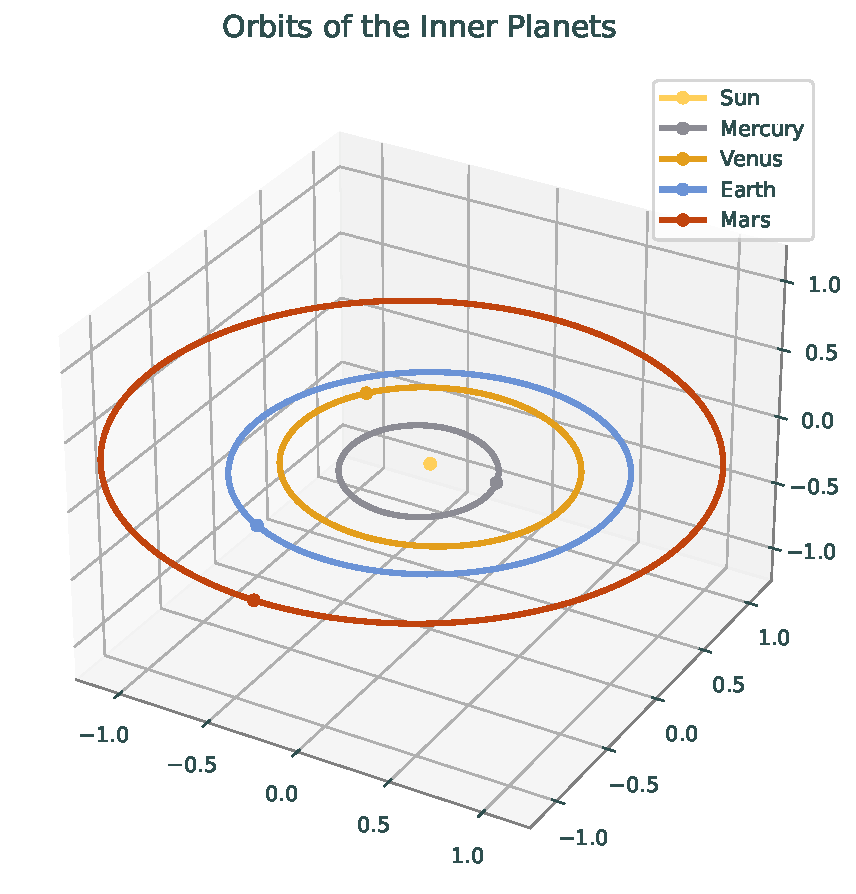
\includegraphics[width=\textwidth]{figures/orbits.png}
\caption{The solution to Problem 2.}
\label{lab0:3dplot}
\end{figure}

\subsection*{3D Animations}
The key difference between 2D and 3D animations is that the \li{.set_data()} method does not support setting the \li{z} values.
Instead, set the \li{x} and \li{y} values with \li{.set_data()} as before, and then set the \li{z} values with \li{.set_3d_properties()}.
The \li{.set_3d_properties()} function call is also made inside the update function. 

Animation in 3D requires more careful consideration than in the 2D case.
When \li{matplotlib} displays a 3D plot, it does so in an interactive figure that allows the user to change the camera angle and position.
Since 3D rendering is more computationally expensive than 2D rendering, interactive views of 3D animations often have poor framerates and choppy rendering.
This is what calling \li{plt.plot()} attempts to do; instead, it is much better to either render the animation to a file and then embed the file, or to use the HTML5 API to embed it, as discussed above.

\begin{problem}
Each row of the arrays in \li{orbits.npz} gives the position of the planets at evenly spaced time points. The arrays correspond to 1400 points in time over a 700 day period (beginning on 2018-5-30).
Create a 3D animation of the planet orbits.
Display lines for the trajectories of the orbits and points for the current positions of the planets at each point in time.
Your \li{update()} function will need to return a list of Line3D objects, one for each orbit trajectory and one for each planet position marker.
Embed your animated plot.
\end{problem}

\section*{Surface Plotting}
3D surface plotting is very similar to regular 3D plotting discussed earlier.
The difference with surface plots is that they require first creating a \textit{meshgrid} for X and Y. Meshgrids are created using the NumPy command \li{np.meshgrid(x, y)} where \li{x} and \li{y} are 1D arrays representing the x and y coordinates of the grid.
This function creates 2D arrays \li{X} and \li{Y} that combined give cartesian cordinates for every point made from the \li{x} and \li{y} arrays. 

Once a meshgrid is defined, a surface plot is generated by calling \li{ax.plot_surface(X, Y, Z)}, where \li{Z} is a 2D array of height values that is the same shape as \li{X} and \li{Y}. 

\begin{problem}
Make a surface plot of the bivariate normal density function given by:

$$f(\mathbf{x})=\frac{1}{\sqrt{det(2\pi \Sigma)}}\exp{\left[-\frac{1}{2}(\mathbf{x} - \mu)^T \Sigma^{-1} (\mathbf{x} - \mu)\right]}$$

where $\mathbf{x}=[x,y]^T$, $\mu=[0,0]^T$ is the mean vector, and $$\Sigma = \begin{bmatrix} 1 & 3/5 \\ 3/5 & 2 \end{bmatrix}$$ is the covariance matrix. Compare your results with Figure \ref{lab0:surf}.
\end{problem}

\begin{figure}[H]
\centering
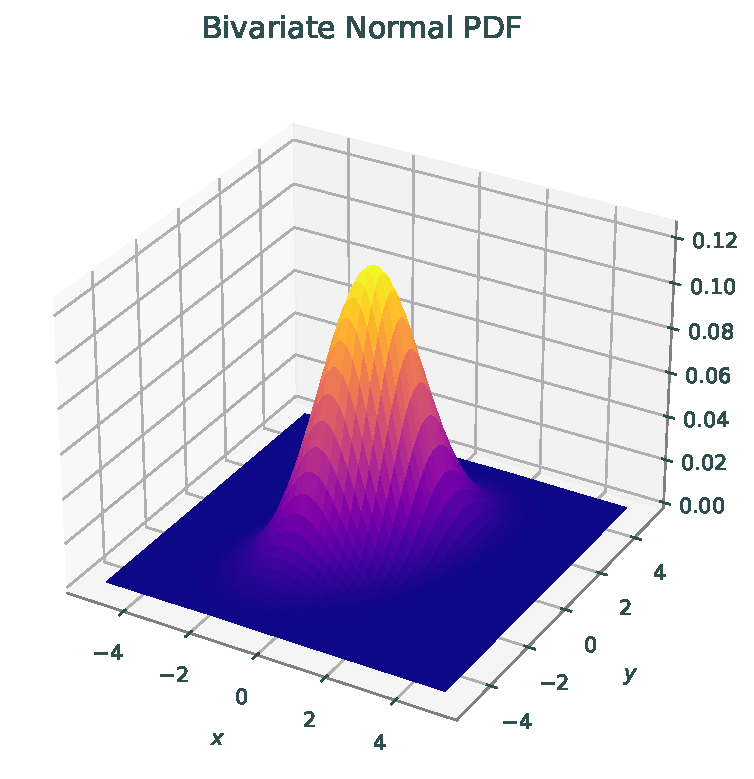
\includegraphics[width=100mm]{figures/normal_density.png}
\caption{The solution to Problem 4.}
\label{lab0:surf}
\end{figure}

\subsection*{Surface Animations}
Animating a 3D surface is slightly different from animating a parametric curve in 3D.
The object created by \li{.plot_surface()} does not have a \li{.set_data()} method.
Instead, use \li{ax.clear()} to empty the axes at each frame, followed by a new call to \li{ax.plot_surface()}.
Note that the axes limits must be reset after \li{ax.clear()} is called. 

\begin{problem}
Use the data in \li{vibration.npz} to produce a surface animation of the solution to the wave equation for an elastic rectangular membrane.
The file contains three NumPy arrays: \li{X}, \li{Y}, \li{Z}.
\li{X} and \li{Y} are meshgrids of shape \li{(300,200)} corresponding to 300 points in the y-direction and 200 points in the x-direction, giving a 2x3 rectangle with one corner at the origin.
\li{Z} is of shape \li{(150,300,200)}, giving the height of the vibrating membrane at each (x,y) point for 150 values of time. 
In the language of partial differential equations, this is the solution to the following initial/boundary value problem:

$$u_{tt} = 6^2(u_{xx}+u_{yy})$$
$$(x,y) \in [0,2]\times[0,3], t \in [0,5]$$
$$u(t,0,y)=u(t,2,y)=u(t,x,0)=u(t,x,3) = 0$$
$$u(0,x,y) = xy(2-x)(3-y)$$
\end{problem}